\chapter{Renormalización, naturalidad y problema de jerarquías}

\lectureoverview{Las ideas centrales de este curso surgieron de cuestiones sobre la renormalización en el Modelo Estándar. Por eso comenzamos por el significado físico de la renormalización: eliminar los grados de libertad que son demasiado pequeños y rápidos para la cuestión que nos ocupa y, después, codificar sus efectos en una descripción efectiva. Una molécula nos proporciona el modelo. El análisis dimensional lleva luego el mismo razonamiento a la teoría cuántica de campos escalares, donde pone de manifiesto la sensibilidad cuadrática de la masa de un escalar, el problema de jerarquías del campo de Higgs, la protección de la que gozan los fermiones y los bosones gauge, y el problema aún más grave de la energía del vacío.}

\section{La física a la escala de la pregunta}

La mayoría de las ideas que desarrollaremos este trimestre surgieron de preguntas sobre la renormalización---a veces desconcertantes, a veces observaciones útiles---en el Modelo Estándar. La renormalización combina dos hábitos de pensamiento. El primero consiste en eliminar de una descripción las estructuras a distancias tan cortas que resultan irrelevantes para la pregunta planteada. El segundo es el análisis dimensional, que a menudo permite determinar la respuesta a distancias cortas antes de evaluar cualquier integral difícil.

Esta eliminación de detalles ocurre en toda la física. Si queremos entender un núcleo, podemos empezar por los quarks y la cromodinámica cuántica. Después de calcular las masas y los espines del protón y el neutrón, junto con sus fuerzas nucleares efectivas, podemos prescindir de su subestructura de quarks para muchos fines. El movimiento nuclear es lo bastante lento como para que una mecánica cuántica no relativista de protones y neutrones sea a menudo la descripción más útil.

En el siguiente nivel, la física atómica normalmente no necesita conocer la constitución interna de un núcleo. La física nuclear nos dice qué núcleos e isótopos existen y proporciona propiedades como la masa y la carga eléctrica. Entonces empezamos de nuevo con un conjunto nuevo de objetos elementales efectivos: núcleos y electrones. Los quarks, protones y neutrones no han dejado de existir; sus efectos se han condensado en los parámetros que llevan los núcleos.

La cantidad de información que conservamos depende de la pregunta siguiente. Un cálculo atómico puede necesitar la masa nuclear, porque interviene en la masa reducida, y sin duda necesita la carga, porque esta determina el campo de Coulomb. Por lo general, no hace falta saber qué quark lleva cada fracción del momento nuclear. Hay unas noventa cargas elementales, y el número de especies nucleares aumenta al contar los isótopos. Ese catálogo puede darse como dato de entrada. Los electrones, en cambio, todavía no se pueden eliminar: su movimiento es precisamente lo que da lugar a la estructura atómica.

Una vez resuelto el problema atómico, podemos considerar, de manera análoga, los átomos como los bloques constituyentes de las moléculas. La lista caprichosa de Susskind —átomos de galleta, átomos de café, átomos de chocolate y átomos de kétchup— transmite una idea seria: cada nivel requiere una descripción nueva. Una vez conocidas las propiedades y las fuerzas moleculares, las moléculas pueden unirse para formar ensamblajes más grandes, como piezas de un juego de construcción, sin tener que volver a plantear el problema de los electrones a cada paso.

Cada paso de este tipo es una coarse-graining, o descripción a escala más gruesa. El nuevo relato puede ser menos exacto en términos absolutos, pero resulta mucho más útil en la escala para la que está destinado. La teoría cuántica de campos hace ineludible esta cuestión, porque un campo tiene modos de todas las longitudes de onda, incluidas las arbitrariamente cortas. Por eso sumamos los efectos de las longitudes de onda demasiado cortas para resolverlas y las reemplazamos por nuevos parámetros efectivos. Esa operación, junto con el análisis dimensional, constituye el contenido físico de la renormalización.

\section{Una molécula como modelo}

Consideremos dos átomos y busquemos una descripción sencilla de su movimiento relativo. Cada átomo contiene un núcleo pesado y una nube de electrones. Incluso el protón tiene una masa aproximadamente dos mil veces mayor que la del electrón, y los núcleos más pesados aumentan la separación entre escalas. Una imagen útil es la de dos bolas de bolos rodeadas de moscas que vuelan rápidamente: los núcleos responden con lentitud mientras el estado electrónico se reorganiza deprisa.

Sean \(R_a\) y \(P_a\) las posiciones y los momentos nucleares, con masa común \(M\), y sean \(r_i\) y \(q_i\) las coordenadas y los momentos de los electrones, de masa \(m_e\). Omitiendo factores convencionales como \(4\pi\epsilon_0\), el hamiltoniano tiene la forma esquemática
\begin{align}
H={}&
\frac{P_1^2}{2M}+\frac{P_2^2}{2M}
+\frac{e^2}{R_{12}}
+\sum_i\frac{q_i^2}{2m_e}
+\frac12\sum_{i\ne j}\frac{e^2}{r_{ij}}
\nonumber\\
&-\sum_i\left(
\frac{e^2}{|R_1-r_i|}
+\frac{e^2}{|R_2-r_i|}
\right).
\label{eq:molecular-hamiltonian}
\end{align}
La primera línea contiene las energías cinéticas nucleares, la repulsión de Coulomb entre los núcleos y la energía cinética electrónica. La segunda línea incluye la repulsión entre electrones y la atracción entre electrones y núcleos. Para núcleos con cargas arbitrarias, se restituyen los factores correspondientes de \(Z_a\); en la clase las cargas se mantienen esquemáticas porque lo que importa es la separación de escalas temporales.

Hay dos tipos de movimiento característicos. Los núcleos son pesados y lentos; los electrones son ligeros y rápidos, tanto que parecen borrosos. En primera aproximación, fijamos las posiciones nucleares y agrupamos todos los términos que dependen de los electrones en un hamiltoniano electrónico,
\begin{equation}
H_{\mathrm{el}}(R_1,R_2).
\end{equation}
Para cada configuración nuclear fija, resolvemos
\begin{equation}
H_{\mathrm{el}}(R_1,R_2)
\psi_0(r_1,\ldots,r_N;R_1,R_2)
=
E_{\mathrm{el}}(R_1,R_2)\psi_0.
\label{eq:electronic-ground-state}
\end{equation}
Conservamos el menor autovalor electrónico. No hemos ignorado los electrones; todo su movimiento rápido queda resumido en la función \(E_{\mathrm{el}}(R_1,R_2)\).

El razonamiento es adiabático. Durante un ajuste electrónico rápido, los núcleos se desplazan tan poco que sus coordenadas pueden tratarse como parámetros. Una vez resuelto el problema de autovalores electrónicos, esas mismas coordenadas vuelven a poder moverse. En cada configuración que cambia lentamente, la nube electrónica sigue su estado fundamental instantáneo. Un tratamiento más preciso podría conservar las superficies electrónicas excitadas y las transiciones entre ellas, pero la superficie principal ya muestra la idea de la renormalización.

\begin{figure}[htbp]
\centering
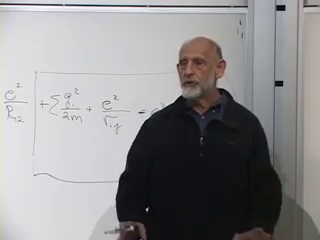
\includegraphics[width=0.72\textwidth]{lecture_01_figure_02.png}
\caption{El hamiltoniano molecular permanece en la pizarra mientras se introduce el problema del estado fundamental electrónico. La expresión mecanografiada en la ecuación~\eqref{eq:molecular-hamiltonian} recoge los términos que esta imagen no deja ver.}
\lectureframe{00:16:19}
\end{figure}

\begin{classroomqa}
\audiencequestion{¿Se están fijando sin más a cero los momentos nucleares?\lecturetimestamp{00:15:39}}
\lecturerresponse{Solo temporalmente. En la aproximación principal, los núcleos se tratan como si estuvieran clavados, porque se mueven mucho más despacio que los electrones. Recuperaremos sus momentos al resolver el problema nuclear efectivo, así que esta aproximación no viola el principio de incertidumbre.}
\end{classroomqa}

La energía del estado fundamental electrónico contribuye ahora al potencial que sienten los núcleos:
\begin{equation}
V_{\mathrm{eff}}(R_1,R_2)
=\frac{e^2}{R_{12}}+E_{\mathrm{el}}(R_1,R_2).
\label{eq:molecular-effective-potential}
\end{equation}
La invariancia rotacional y traslacional hace que, para dos átomos aislados, dependa solo de su separación \(R_{12}\). A distancias muy cortas domina la repulsión de Coulomb entre los núcleos. A distancias muy grandes, la interacción es pequeña. Entre esos límites, la nube electrónica puede producir una región atractiva y un mínimo. La función de onda nuclear se concentra entonces cerca de ese mínimo y describe una molécula ligada.

Fijémonos en el orden de las operaciones. No supusimos una atracción empírica para descartar luego los electrones. Primero resolvimos su problema cuántico en el fondo de núcleos fijos. Solo entonces eliminamos sus coordenadas explícitas y conservamos el autovalor resultante. La física de distancias cortas sobrevive en la forma, la profundidad y la curvatura de \(V_{\mathrm{eff}}\). La posición de su mínimo determina la separación de equilibrio, su curvatura controla las pequeñas vibraciones y su forma asintótica determina si existe un estado ligado. Una sola función efectiva lleva toda esa información electrónica al problema más lento.

Así, un hamiltoniano complicado de muchos electrones se ha convertido en un hamiltoniano nuclear de dos cuerpos con un potencial nuevo. Hemos eliminado los grados de libertad rápidos, pero conservado todo su efecto a baja energía. El potencial ha sido renormalizado. Este razonamiento familiar de Born--Oppenheimer no suele presentarse con ese nombre, pero contiene exactamente la idea que necesitamos:
\begin{equation}
\begin{gathered}
\text{fast microscopic dynamics}\\
\Downarrow\\
\text{effective parameters for slow dynamics}
\end{gathered}
\end{equation}

\section{Unidades naturales y dimensión de un campo}

En teoría cuántica de campos, los modos que se eliminan pueden describirse indistintamente como modos de distancias cortas, longitudes de onda cortas, frecuencias altas o energías altas. Antes de dibujar diagramas, establezcamos la contabilidad dimensional.

La mecánica ordinaria usa unidades independientes de longitud, tiempo y masa. En física de partículas fijamos
\begin{equation}
\hbar=c=1.
\end{equation}
Entonces, energía y masa son equivalentes por \(E=mc^2\), longitud y tiempo lo son porque \(c=1\), y \(\hbar=1\) hace que el momento sea el inverso de la longitud. Solo queda una dimensión:
\begin{equation}
[M]=[E]=[p]=L^{-1},
\qquad
[x]=[t]=L.
\label{eq:natural-units}
\end{equation}

Esto no elimina las dimensiones. Elige factores de conversión de modo que el tiempo pueda expresarse como una longitud y la masa como el inverso de una longitud. Una vez especificada una unidad, todas las demás se deducen. Por eso un corte puede describirse como una distancia corta \(\delta\) o como una energía alta \(\Lambda=1/\delta\): son la misma escala expresada en dos lenguajes.

Consideremos un campo escalar real \(\phi\), con una densidad lagrangiana normalizada esquemáticamente,
\begin{equation}
\mathcal L=(\partial_\mu\phi)(\partial^\mu\phi)-V(\phi),
\qquad
S=\int d^4x\,\mathcal L.
\label{eq:scalar-action}
\end{equation}

\begin{figure}[htbp]
\centering
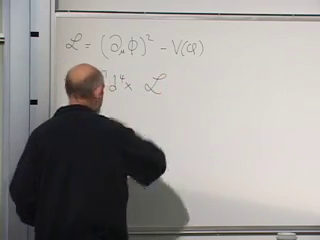
\includegraphics[width=0.78\textwidth]{lecture_01_figure_03.png}
\caption{La densidad lagrangiana escalar local y su integral sobre el espacio-tiempo, que da la acción.}
\lectureframe{00:26:08}
\end{figure}

La densidad lagrangiana es local: describe un punto del espacio-tiempo. Las ecuaciones clásicas de campo se obtienen haciendo estacionaria la acción. En teoría cuántica, la misma acción aparece en la fase de la integral de caminos \(\exp(iS)\). En cualquiera de los dos enfoques, la dimensión de \(S\) es decisiva. Al restituir \(\hbar\), la fase es \(\exp(iS/\hbar)\); una vez fijado \(\hbar=1\), \(S\) debe ser adimensional.

\begin{classroomqa}
\audiencequestion{¿La acción tiene unidades de \(\hbar\)?\lecturetimestamp{00:26:13}}
\lecturerresponse{Sí. Como se ha fijado \(\hbar\) igual a uno, en estas unidades la acción es adimensional. La medida cuatridimensional tiene dimensión \(L^4\), así que la densidad lagrangiana debe tener dimensión \(L^{-4}\).}
\end{classroomqa}

El término cinético fija ahora la dimensión del campo:
\begin{align}
[S]&=1, & [\mathcal L]&=L^{-4},\\
[\partial_\mu]&=L^{-1}, &
[(\partial\phi)^2]&=L^{-2}[\phi]^2=L^{-4},\nonumber\\
&& [\phi]&=L^{-1}.
\label{eq:scalar-dimension}
\end{align}
Este breve cálculo determinará el comportamiento ultravioleta de todos los diagramas que siguen.

Desarrollemos el potencial como
\begin{equation}
V(\phi)=\frac{m^2}{2}\phi^2+g\phi^3+\lambda\phi^4+\cdots.
\label{eq:scalar-potential}
\end{equation}
Todos los términos deben tener dimensión \(L^{-4}\). Como
\([\phi^n]=L^{-n}\),
\begin{equation}
[m^2]=L^{-2},
\qquad
[g]=L^{-1},
\qquad
[\lambda]=1.
\label{eq:coupling-dimensions}
\end{equation}
El acoplamiento cuártico es adimensional. Estos acoplamientos son especialmente importantes en la renormalización porque su dependencia de la escala no se deduce de una simple potencia de la longitud.

\begin{classroomqa}
\audiencequestion{¿\(g\) tiene unidades de masa?\lecturetimestamp{00:29:52}}
\lecturerresponse{Sí. El factor \(\phi^3\) tiene dimensión \(L^{-3}\), mientras que la densidad del potencial debe tener dimensión \(L^{-4}\). Por tanto, \([g]=L^{-1}\), que en unidades naturales es una masa.}
\end{classroomqa}

\section{Vértices y propagador a distancias cortas}

Las reglas de Feynman se construyen a partir de vértices y propagadores. El término \(g\phi^3\) da un vértice de tres líneas con un factor proporcional a \(g\); \(\lambda\phi^4\) da un vértice de cuatro líneas con un factor proporcional a \(\lambda\). El término cuadrático da una inserción local de dos puntos. Puede representarse como una partícula que entra, es absorbida y vuelve a emitirse, con un coeficiente proporcional a \(m^2/2\). Se omiten deliberadamente las normalizaciones numéricas, los signos, los factores de \(i\) y los factores de simetría, porque la clase busca extraer la dependencia de escala, no calcular una sección eficaz.

Estos dibujos tienen una interpretación operativa. Un vértice de tres puntos puede absorber dos cuantos y emitir uno, o representar cualquier asignación de sus tres líneas relacionada por cruce. Un vértice de cuatro puntos puede describir dos partículas que entran y dos que salen. La cruz cuadrática sigue siendo un vértice legítimo de dos líneas, aunque normalmente se incorpore al propagador libre. La mostramos porque pronto identificaremos todo proceso de dos puntos no resuelto comparándolo con ella.

Un propagador conecta dos puntos del espacio-tiempo. Su línea no afirma que una partícula cuántica haya seguido una trayectoria clásica rectilínea. Representa la amplitud de crear una excitación del campo en \(x\) y eliminarla o detectarla en \(y\):
\begin{equation}
\Delta(x-y)=\langle0|\phi(y)\phi(x)|0\rangle.
\label{eq:position-propagator}
\end{equation}
Leamos la expresión de derecha a izquierda. Al actuar sobre el vacío, \(\phi(x)\) crea una componente de una partícula en \(x\). Al actuar sobre el bra, \(\phi(y)\) elimina la componente en \(y\). Su elemento de matriz entre estados de vacío es la amplitud de solapamiento entre la creación en el primer punto y la detección en el segundo. Los símbolos \(x\) y \(y\) representan cuatro-vectores completos, no solo dos coordenadas cartesianas.

Los estados no tienen dimensión física, mientras que cada campo aporta \(L^{-1}\). Por tanto,
\begin{equation}
[\Delta]=L^{-2}.
\end{equation}
Para un campo sin masa no hay una escala intrínseca de longitud, así que el análisis dimensional impone el comportamiento a distancias cortas
\begin{equation}
\Delta(x-y)\sim\frac{1}{(x-y)^2}.
\label{eq:massless-propagator}
\end{equation}
El denominador es la separación al cuadrado invariante de Lorentz, con la prescripción usual necesaria en sus singularidades.\editorialnote{Para el conteo de potencias resulta conveniente hacer una rotación de Wick a una separación euclídea, donde el módulo es inequívocamente proporcional a \(1/|x-y|^2\). Esto no cambia las potencias ultravioletas que usaremos a continuación.}

Cuando \(y\) se aproxima a \(x\), el propagador diverge. Esta singularidad de la propagación a través de una separación que se anula es el origen de las divergencias ultravioletas que aparecen en diagramas más elaborados.

\section{Cómo se renormaliza la masa de un escalar}

Para un campo escalar, el parámetro dinámico es \(m^2\), como ya sugiere la relación de dispersión relativista:
\begin{equation}
E=\sqrt{\mathbf p^2+m^2}.
\end{equation}
Sea \(\delta\) la distancia más corta que resuelve nuestra descripción efectiva. No distinguiremos los procesos cuyos vértices estén separados por menos de \(\delta\). Cualquier proceso no resuelto de ese tipo, con un escalar entrante y otro saliente, tiene la misma forma observable de dos puntos que una inserción de masa y, por tanto, debe contribuir a la masa efectiva.

Pensemos en un acelerador como en un microscopio. Si su resolución más fina es \(\delta\), una absorción en un punto seguida de una emisión a una distancia mucho menor que \(\delta\) no puede distinguirse de un suceso verdaderamente local. Difuminamos deliberadamente el vértice a esa escala. La renormalización es la regla que incorpora todas esas alternativas por debajo de la resolución al coeficiente del operador local correspondiente.

\subsection{Primera corrección cuártica}

Empecemos con un único vértice \(\phi^4\). Dos líneas corresponden a la partícula externa; las otras dos se unen para formar un bucle corto que se emite y se reabsorbe casi en el mismo punto. Al promediar el propagador coincidente en la distancia de corte, obtenemos
\begin{equation}
\Delta(0)\ \longrightarrow\ \Delta(\delta)\sim\frac{1}{\delta^2},
\end{equation}
y, por tanto,
\begin{equation}
\delta m^2_{(1)}\sim\frac{\lambda}{\delta^2}.
\label{eq:one-loop-scalar-mass}
\end{equation}
Si \(m_0^2\) denota el parámetro de entrada o desnudo, el coeficiente de dos puntos a baja resolución tiene la forma esquemática
\begin{equation}
\frac{m_{\mathrm{eff}}^2}{2}
\sim
\frac{m_0^2}{2}
+c_1\frac{\lambda}{\delta^2},
\label{eq:first-renormalized-mass}
\end{equation}
donde \(c_1\) recoge los factores numéricos y dependientes de la convención que se han omitido. La masa de laboratorio medida en experimentos que no resuelven distancias menores que \(\delta\) es esta cantidad renormalizada, no \(m_0\) por sí sola.

Hay, por tanto, dos maneras indistinguibles de que ocurra el suceso observado de dos puntos. El vértice cuadrático original puede absorber y reemitir la partícula, o la interacción cuártica puede hacerlo tras emitir y reabsorber brevemente un escalar virtual. La mecánica cuántica suma las amplitudes. Cuando el bucle queda por debajo de la escala de resolución, su historia por separado desaparece de la descripción efectiva, pero su contribución al coeficiente medido permanece.

\subsection{Siguiente corrección cuártica}

Conectemos ahora dos vértices cuárticos de modo que una partícula externa entre en \(x\), otra salga de \(x+\Delta\) y tres propagadores internos unan los vértices. Hay dos potencias de \(\lambda\), mientras que los propagadores aportan \(\Delta^{-6}\). Las amplitudes cuánticas deben sumarse sobre todos los puntos no resueltos de los que puede emerger la partícula saliente, así que se integra el cuatro-vector relativo:
\begin{equation}
\delta m^2_{(2)}
\sim
\lambda^2
\int_{|\Delta|\gtrsim\delta}
d^4\Delta\,\frac{1}{|\Delta|^6}.
\label{eq:two-loop-power-count}
\end{equation}

\begin{classroomqa}
\audiencequestion{¿La pequeña marca en el vértice significa que allí solo hay tres partículas?\lecturetimestamp{00:46:35}}
\lecturerresponse{No. Seguimos usando la interacción cuártica. En cada vértice se encuentran cuatro líneas; en este diagrama de dos puntos, una es externa y tres van de un vértice al otro. El segundo vértice también tiene cuatro líneas incidentes.}
\end{classroomqa}

La medida aporta cuatro potencias de longitud y los tres propagadores, menos seis. Como el corte ultravioleta es la única escala de la estimación,
\begin{equation}
\int_{|\Delta|\gtrsim\delta}
\frac{d^4\Delta}{|\Delta|^6}
\sim\frac{1}{\delta^2},
\qquad
\delta m^2_{(2)}
\sim\frac{\lambda^2}{\delta^2}.
\label{eq:two-loop-scalar-mass}
\end{equation}
Aquí \(\Delta^\mu\) es una variable de integración de cuatro componentes; se integra sobre su componente temporal y sus tres componentes espaciales. La \(\delta\) minúscula es el corte fijo. Al principio, en la exposición oral se usa el mismo nombre para ambas y más adelante se corrige la notación.

El mismo resultado se ve al expresar radialmente la medida cuatridimensional. Salvo una constante angular,
\begin{equation}
\int_{\delta}\frac{d^4\Delta}{|\Delta|^6}
\sim
\int_{\delta}\frac{R^3\,dR}{R^6}
=\int_{\delta}\frac{dR}{R^3}
\sim\frac{1}{\delta^2}.
\end{equation}
Por eso el límite superior de distancias grandes no importa para la estimación ultravioleta: la integral está dominada por su extremo inferior.

Los diagramas de orden superior repiten el patrón. Un diagrama con más vértices cuárticos añade una potencia mayor de \(\lambda\), pero el análisis dimensional sigue permitiendo una contribución cuadráticamente divergente a la masa:
\begin{equation}
\begin{aligned}
m_{\mathrm{eff}}^2
={}&m_0^2
+\frac{1}{\delta^2}
\left(c_1\lambda+c_2\lambda^2+c_3\lambda^3+\cdots\right)\\
&+\text{weaker terms}.
\end{aligned}
\label{eq:scalar-mass-series}
\end{equation}

\subsection{La interacción cúbica y un logaritmo}

Dos vértices cúbicos contienen dos propagadores entre puntos cercanos. Su contribución escala como
\begin{equation}
\delta m_g^2
\sim
g^2\int_{|\Delta|\gtrsim\delta}
\frac{d^4\Delta}{|\Delta|^4}.
\label{eq:cubic-loop}
\end{equation}
Ahora, la medida y el denominador llevan las mismas potencias. La dependencia restante es logarítmica, en lugar de ser una potencia:
\begin{equation}
\delta m_g^2
\sim
c_g g^2\log\!\left(\frac{1}{\mu\delta}\right).
\label{eq:cubic-log}
\end{equation}
La escala de referencia \(\mu\) hace que el logaritmo sea adimensional. Esta es la versión con dimensiones correctas de la expresión esquemática de la clase \(g^2\log\delta\). Un logaritmo varía mucho más lentamente que cualquier potencia inversa, así que \(1/\delta^2\) domina cuando el corte corresponde a distancias cortas.

De nuevo, la forma radial hace patente la diferencia:
\begin{equation}
\int_{\delta}^{R_{\mathrm{IR}}}
\frac{d^4\Delta}{|\Delta|^4}
\sim
\int_{\delta}^{R_{\mathrm{IR}}}\frac{R^3\,dR}{R^4}
=\log\!\left(\frac{R_{\mathrm{IR}}}{\delta}\right).
\end{equation}
La igualdad de potencias en la medida y el denominador produce un logaritmo. Si el denominador tiene más potencias, se obtiene una potencia inversa del corte. La clase no nos pide evaluar los factores angulares; nos enseña a reconocer a simple vista la respuesta ultravioleta.

\begin{classroomqa}
\audiencequestion{¿Cuál es la base del logaritmo?\lecturetimestamp{00:57:42}}
\lecturerresponse{Se usa el logaritmo natural. Cambiar la base solo lo multiplica por una constante numérica, que queda absorbida en el coeficiente cuyos factores de \(2\), \(\pi\) y simetría no se han calculado aquí.}
\end{classroomqa}

\begin{classroomqa}
\audiencequestion{¿Cómo se puede tomar el logaritmo de una longitud y de dónde salen las unidades de la corrección de masa?\lecturetimestamp{00:58:32}}
\lecturerresponse{Un logaritmo siempre compara dos escalas; rigurosamente, es el logaritmo de una razón adimensional, como \(1/(\mu\delta)\). El acoplamiento \(g\) tiene una potencia de masa, así que \(g^2\) ya tiene exactamente la dimensión de masa al cuadrado que requiere la corrección.}
\end{classroomqa}

\begin{classroomqa}
\audiencequestion{Un diagrama de Feynman da una amplitud. ¿Su módulo al cuadrado es una probabilidad?\lecturetimestamp{00:59:41}}
\lecturerresponse{Sí, cuando la amplitud se incluye en un cálculo de una transición física con los factores de estado y de espacio de fases necesarios. Aquí su función más inmediata es distinta: una amplitud de dos puntos no resuelta tiene la misma forma local que el término de masa y, por tanto, modifica el parámetro de masa efectivo.}
\end{classroomqa}

\section{Todos los parámetros se vuelven efectivos}

La familia infinita de diagramas de masa no desaparece simplemente porque \(\lambda\) sea pequeño. La teoría de perturbaciones los ordena por potencias del acoplamiento, de modo que los términos sucesivos pueden ser menores, pero siguen siendo infinitos. La misma eliminación de procesos a distancias cortas también renormaliza las propias interacciones.

\begin{classroomqa}
\audiencequestion{¿No hay también infinitos diagramas incluso para la renormalización de la masa?\lecturetimestamp{01:00:35}}
\lecturerresponse{Sí. Si \(\lambda\) es lo bastante pequeño, la serie perturbativa puede ser útil porque las potencias sucesivas quedan cada vez más suprimidas. Sin embargo, el parámetro renormalizado se define mediante la serie completa, no solo por el primer dibujo.}
\end{classroomqa}

Desde el punto de vista operativo, una interacción local \(\lambda\phi^4\) es una amplitud con dos partículas entrantes y dos salientes. Si un proceso de cuatro puntos más complicado ocurre por entero en una región no resuelta, a baja resolución no se distingue del vértice local original. Por ello, esos diagramas se agrupan en un \(\lambda\) efectivo. En una teoría \(\phi^4\) cuatridimensional, su dependencia principal de la escala suele ser logarítmica. La clase no calcula esa función beta; usa el ejemplo para enunciar la idea general:
\begin{equation}
\begin{gathered}
\text{parameters measured at low energy}\\
\ne\\
\text{parameters entered at the microscopic cutoff}
\end{gathered}
\end{equation}

El ejemplo de cuatro puntos importa porque disipa un posible malentendido. La renormalización no es un arreglo especial que se aplica solo a la divergencia de masa. Todo operador permitido en la lagrangiana puede reproducirse mediante diagramas no resueltos con las mismas líneas externas y simetrías. Un proceso de dos puntos renormaliza un coeficiente cuadrático, uno de cuatro puntos renormaliza un coeficiente cuártico y los procesos de vacío a vacío renormalizan el término constante. La lagrangiana de baja energía es el registro compacto donde quedan asentados todos esos procesos a distancias cortas.

\begin{classroomqa}
\audiencequestion{Como \(\Delta\) tiene unidades de longitud, ¿no resulta dimensionalmente extraño tomar su logaritmo? ¿Y se intercambiaron en la pizarra las deltas mayúscula y minúscula?\lecturetimestamp{01:01:34}}
\lecturerresponse{El logaritmo se refiere en realidad a una razón respecto de otra escala y, por tanto, es adimensional. Sí, la notación se intercambió brevemente: \(\Delta^\mu\) es la variable de integración, mientras que \(\delta\) es el corte inferior de distancia que permanece en el resultado.}
\end{classroomqa}

Este es el equivalente en teoría de campos de la molécula. Resolvimos el problema de los electrones rápidos que no observamos e incorporamos el resultado a un potencial. Aquí sumamos los procesos a distancias cortas que no observamos e incorporamos el resultado a las masas, los acoplamientos y todos los demás coeficientes locales permitidos. Todo se modifica.

\begin{classroomqa}
\audiencequestion{¿Podría repetir si la cantidad medida incluye las escalas menores que las que el experimento puede detectar?\lecturetimestamp{01:05:13}}
\lecturerresponse{Sí. Sus fluctuaciones individuales no se resuelven, pero su efecto acumulado está presente. Todos los diagramas que involucran escalas más cortas se agrupan en el único coeficiente efectivo al que un experimento de baja energía llama, por ejemplo, masa física al cuadrado.}
\end{classroomqa}

\begin{classroomqa}
\audiencequestion{¿Debe entonces el término de entrada \(m_0^2\) cancelar las demás contribuciones?\lecturetimestamp{01:06:00}}
\lecturerresponse{Si la masa escalar medida es mucho menor que las contribuciones ultravioletas individuales, sí. La cancelación necesaria es el problema del ajuste fino que abordaremos ahora.}
\end{classroomqa}

\section{El problema de jerarquía del Higgs}

Imaginemos que el corte es la longitud de Planck, de modo que se pide a la teoría efectiva de campos que resuma las fluctuaciones desde las escalas de laboratorio hasta la escala en que debe intervenir la gravedad cuántica.
En unidades de física de partículas,
\begin{equation}
\delta\sim M_{\mathrm{Pl}}^{-1}\sim10^{-19}\,\mathrm{GeV}^{-1},
\qquad
\frac{1}{\delta^2}\sim10^{38}\,\mathrm{GeV}^2.
\label{eq:planck-cutoff}
\end{equation}
Para esta enorme comparación, no importa si se usa la escala de Planck reducida o la no reducida.

La jerarquía de distancias resulta igualmente sorprendente. La longitud de Planck es unos diecinueve órdenes de magnitud menor que el radio del protón y aproximadamente dieciséis o diecisiete órdenes de magnitud menor que las distancias exploradas directamente por los aceleradores mencionados. Al elevar esa separación al cuadrado se obtiene la cancelación de unas treinta y cuatro cifras en un parámetro escalar de masa al cuadrado.

Para el campo de Higgs, que es un escalar, la escala electrodébil deseada es del orden de unos cientos de GeV, no de \(10^{19}\) GeV. Sin embargo, los términos de la ecuación~\eqref{eq:scalar-mass-series} pueden tener de manera natural el orden de magnitud de la escala de Planck.
No se han determinado sus signos: algunos pueden ser positivos y otros negativos, y la masa desnuda al cuadrado también puede tener cualquiera de los dos signos. Pero, para que quede un residuo de escala electrodébil, esas contribuciones enormes deben cancelarse hasta unas treinta y cuatro cifras decimales. Susskind primero dice diecisiete cifras y luego se corrige, porque la comparación es entre masas al cuadrado. En esta versión del ajuste, lo que mide la magnitud del ajuste es la razón al cuadrado.

\begin{classroomqa}
\audiencequestion{¿Es \(\lambda\) menor o mayor que uno?\lecturetimestamp{01:09:50}}
\lecturerresponse{Se supone que es algo menor que uno. La teoría de perturbaciones se volvería intratable si las potencias sucesivas crecieran, y tampoco se puede extrapolar de manera consistente una teoría puramente escalar con un acoplamiento cuártico arbitrariamente grande. Pero \(\lambda\) no es ni de lejos tan pequeña como \(10^{-38}\); para orientarse, la conferencia toma un valor del orden de un porcentaje.}
\end{classroomqa}

\begin{classroomqa}
\audiencequestion{Aunque \(\lambda<1\), ¿no siguen siendo importantes muchos términos porque cada uno lleva el gran factor de corte?\lecturetimestamp{01:10:43}}
\lecturerresponse{Sí. Las potencias superiores acaban suprimiendo la serie, pero antes de que eso ocurra puede contribuir un gran número de términos. Todos ellos, junto con el término desnudo, tendrían que conspirar para dejar como resultado el valor físico extraordinariamente pequeño.}
\end{classroomqa}

Recordemos por qué se sabe que el parámetro de masa del Higgs está en la escala débil. En la convención de la conferencia, escribamos el potencial de ruptura de simetría como
\begin{equation}
V(\phi)=-\frac{\mu^2}{2}\phi^2+\frac{\lambda}{4}\phi^4.
\label{eq:higgs-potential}
\end{equation}
El coeficiente cuadrático negativo hace que el origen sea inestable, mientras que el término cuártico positivo estabiliza el potencial. Al derivar,
\begin{equation}
\frac{dV}{d\phi}=-\mu^2\phi+\lambda\phi^3
=\phi(-\mu^2+\lambda\phi^2),
\end{equation}
se obtiene el mínimo no nulo
\begin{equation}
\phi_{\min}^2=f^2=\frac{\mu^2}{\lambda}.
\label{eq:higgs-minimum}
\end{equation}
En la pizarra se escribe el término cuártico de forma esquemática como \(\lambda\phi^4\), pero se cita la ec.~\eqref{eq:higgs-minimum}; al incluir el factor convencional \(1/4\), ambas expresiones son coherentes sin que cambie el argumento.

El signo de \(-\mu^2\) es importante, pero no resuelve el problema de naturalidad. Lo que provoca la ruptura espontánea de simetría es la curvatura negativa en el origen. La renormalización desplaza esa curvatura mediante contribuciones grandes, tanto positivas como negativas. El vacío roto observado exige que su suma no solo sea pequeña, sino que tenga el valor negativo pequeño preciso que sitúa el mínimo en la escala débil.

Las masas de los bosones \(W\) y \(Z\) determinan que \(f\) sea del orden de \(200\,\mathrm{GeV}\) en la normalización aproximada empleada en la conferencia. Si \(\lambda\) no es ni enorme ni extraordinariamente diminuta, \(\mu\) debe ser del mismo orden general. Por tanto, el coeficiente observado en la escala débil es el residuo de contribuciones que pueden ser, cada una, decenas de órdenes de magnitud mayores.

Esto se conoce como el problema del ajuste fino del Higgs, el problema de jerarquía o el problema de jerarquía gauge. La jerarquía es la enorme razón entre la escala débil ordinaria y una posible escala de unificación o de Planck. Un número pequeño, por sí solo, no tiene por qué resultar paradójico. Lo inquietante aquí es que un número pequeño se forme a partir de contribuciones grandes y aparentemente independientes, que deben cancelarse con una precisión extrema. El problema se reconoció a finales de los 1970 y principios de los 1980, y la búsqueda de un mecanismo que explique esa cancelación motiva la supersimetría y varias ideas alternativas.

La serie perturbativa infinita agudiza el enigma, en vez de eliminarlo. Un valor de \(\lambda\) del orden de un porcentaje hace pequeñas las potencias suficientemente altas, pero antes de que esa supresión prevalezca pueden aparecer muchos términos. No basta con que un lazo cancele por accidente la masa desnuda. La escala débil efectiva debe seguir siendo estable una vez incluidas las demás contribuciones de corta distancia. Una relación estructural entre los términos sería una explicación; una cancelación dígito por dígito entre términos independientes es solo un ajuste fino.

\section{Por qué la masa de un fermión se comporta mejor}

Las demás partículas del Modelo Estándar no requieren ajustes independientes del mismo tipo. Para un fermión de Dirac, el término de masa es
\begin{equation}
\mathcal L_m=-m\bar\psi\psi
=-m\left(\bar\psi_L\psi_R+\bar\psi_R\psi_L\right).
\label{eq:fermion-mass}
\end{equation}
Contiene la masa, no su cuadrado, y acopla las quiralidades izquierda y derecha. Por tanto, una inserción local de masa transforma \(L\) en \(R\), o \(R\) en \(L\).

\begin{figure}[htbp]
\centering
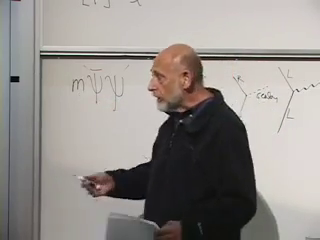
\includegraphics[width=0.76\textwidth]{lecture_01_figure_04.png}
\caption{El término de masa del fermión y los esquemas de la pizarra que muestran cambios de quiralidad. Los diagramas se reconstruyen algebraicamente a continuación, ya que parte del trabajo en la pizarra está oculta.}
\lectureframe{01:23:36}
\end{figure}

En la conferencia oral se suele hablar de lateralidad o helicidad. La protección exacta se expresa con mayor claridad en términos de quiralidad. Para una partícula ultrarrelativista, la imagen de la helicidad aporta la intuición buscada, pero la quiralidad es la propiedad que llevan los campos izquierdos y derechos en la ec.~\eqref{eq:fermion-mass}.

Las interacciones gauge conservan la quiralidad:
\begin{equation}
L\xrightarrow{\ \gamma\ }L,
\qquad
R\xrightarrow{\ \gamma\ }R.
\label{eq:gauge-preserves-chirality}
\end{equation}
Una interacción de Yukawa con un escalar conecta quiralidades opuestas:
\begin{equation}
L\xleftrightarrow{\ \phi\ }R.
\label{eq:scalar-flips-chirality}
\end{equation}
Supongamos primero que el electrón parte de \(m_0=0\). Emitir y reabsorber cualquier número de fotones no puede generar una masa, porque cada vértice gauge conserva la quiralidad. Una secuencia que empieza a la izquierda sigue siendo izquierda. Así, la electrodinámica cuántica pura permite de manera consistente un electrón sin masa: su autoenergía electromagnética no puede generar una masa aditiva a partir de cero.

En la imagen de las líneas, partamos de un electrón de quiralidad izquierda. En el primer vértice con el fotón sigue siendo de quiralidad izquierda; después de propagarse y reabsorber el fotón, también sigue siendo de quiralidad izquierda. Repetir la construcción solo añade más vértices que conservan la quiralidad. Se puede renormalizar la función de dos puntos externa, pero esta no puede adquirir la estructura izquierda-derecha que define una masa.

¿Podría lograrlo la emisión de un escalar? Un vértice escalar transforma \(L\) en \(R\), pero el escalar emitido debe reabsorberse. Por tanto, un diagrama de autoenergía de dos puntos contiene un número par de vértices escalares. El segundo cambio invierte el primero, de modo que el diagrama completo vuelve a conservar la quiralidad externa. Por complicada que se vuelva la gráfica interna, la emisión y la reabsorción emparejan los vértices e impiden que aparezca un término aditivo de \(L\) a \(R\) cuando la masa inicial es cero.

Este es un argumento de paridad sobre el número de cambios. Un vértice escalar cambia la quiralidad una vez; cerrar cada línea escalar interna requiere un segundo extremo y, por tanto, un segundo cambio. Cuatro vértices escalares producen cuatro cambios, y así sucesivamente. Un número par devuelve el fermión a su quiralidad original. La conclusión no se limita al lazo más sencillo dibujado en la pizarra.

Una corrección de masa no nula solo es posible si el diagrama ya contiene una inserción de masa. Por ejemplo, la emisión y reabsorción de un fotón pueden rodear una inserción \(m_0\bar\psi\psi\). Los vértices gauge aportan dos potencias de la carga eléctrica, pero el único cambio de quiralidad aporta la masa original:
\begin{equation}
\begin{aligned}
m_e
&=m_0+c_1e^2m_0+c_2e^4m_0+\cdots\\
&=m_0\left(1+c_1e^2+c_2e^4+\cdots\right).
\end{aligned}
\label{eq:multiplicative-fermion-mass}
\end{equation}
Si \(m_0=0\), el resultado sigue siendo cero. Si \(m_0\) es pequeña, cada corrección es proporcional a ese valor pequeño. Aún podemos preguntarnos por qué el electrón es ligero en relación con una escala fundamental, pero ya no estamos restando números enormes e independientes para obtener su masa. En este sentido, una masa fermiónica pequeña es técnicamente natural.

La inserción de masa hace explícita la secuencia permitida. Empecemos con \(L\). La emisión del fotón conserva \(L\); la inserción \(m_0\) transforma \(L\) en \(R\); la reabsorción del fotón conserva \(R\). Ahora el diagrama tiene la quiralidad externa propia de un término de masa, pero su valor contiene necesariamente el factor \(m_0\). Este es el contraste crucial con la ec.~\eqref{eq:one-loop-scalar-mass}, cuya corrección escalar sigue siendo distinta de cero incluso cuando la masa escalar inicial se fija en cero.

Los bosones gauge cuentan con una protección análoga: la simetría gauge prohíbe un término de masa independiente, por lo que un bosón gauge que parte sin masa permanece sin masa en todos los órdenes perturbativos. En el Modelo Estándar, las masas de los fermiones y de los bosones gauge débiles aparecen en respuesta al valor esperado del Higgs. Si se controla la escala del Higgs, las demás masas pequeñas no requieren copias independientes del mismo ajuste catastrófico.

Esto identifica la cuestión que la supersimetría pretende abordar: ¿puede una teoría impedir que el escalar de Higgs reciba una corrección aditiva de masa enorme? La respuesta es sí en ciertos contextos supersimétricos, porque las contribuciones bosónicas y fermiónicas están relacionadas y no son independientes. El mecanismo detallado comienza en la próxima conferencia.

\section{El otro ajuste fino: la energía del vacío}

Hay otro problema de renormalización aún más grave, pero solo se vuelve observable al incluir la gravedad. En la física no gravitatoria, sumar una constante a todas las energías no cambia ningún experimento. La masa del electrón, por ejemplo, no es una energía absoluta; es la energía adicional necesaria para añadir un electrón al vacío:
\begin{equation}
m_e=E(\text{vacuum}+\text{one electron})-E(\text{vacuum})
\end{equation}
en el sistema de reposo del electrón. Si el vacío y todos los estados excitados se desplazan juntos, sus diferencias no cambian.

Sin embargo, los diagramas de vacío a vacío sí desplazan la energía del vacío. En una teoría \(\lambda\phi^4\), se unen las cuatro patas de un vértice cuártico para formar dos lazos cortos. Cada propagador en coincidencia aporta \(1/\delta^2\), de modo que
\begin{equation}
\delta\rho_{\mathrm{vac}}
\sim
c_{\mathrm{vac}}\frac{\lambda}{\delta^4}.
\label{eq:vacuum-energy-divergence}
\end{equation}
Los diagramas de vacío más complicados llevan distintos factores de acoplamiento y coeficientes, pero el análisis dimensional suele dejar la misma sensibilidad cuártica al corte para la densidad de energía.

La ausencia de líneas externas es precisamente lo que identifica la corrección. Los diagramas de dos puntos comparan un estado de una partícula con el vacío y modifican una masa; los de cuatro puntos modifican la dispersión; un diagrama sin partículas entrantes ni salientes cambia la amplitud de vacío a vacío en sí. Un vértice cuártico aporta \(\lambda\), y sus dos lazos cortos aportan \(\delta^{-2}\) cada uno. El análisis dimensional exige entonces la escala de densidad de energía \(\delta^{-4}\).

Sin gravedad, se puede elegir el cero aditivo de la energía y preguntar a quién le importa. La relatividad general elimina esa libertad: el tensor de energía-momento es fuente de la curvatura del espacio-tiempo, así que una energía uniforme del vacío hace que el espacio vacío gravite. Aparece como una constante cosmológica y se relaciona observacionalmente con la energía oscura. Una energía del vacío medida como diminuta debe sobrevivir entonces a contribuciones de la forma \(\delta^{-4}\).

Por eso cambia la cuestión al activar la gravedad. En la mecánica cuántica ordinaria, desplazar todos los niveles en la misma constante deja intactas todas las frecuencias de transición. En gravedad, la constante no es inerte: el tensor de tensiones del vacío es proporcional a la métrica y curva el espacio-tiempo. Lo que era un cero de energía arbitrario se convierte en una fuente en la ecuación de Einstein.

Así pues, hay al menos dos problemas extremos de naturalidad. La conferencia cita aproximadamente 123 decimales de ajuste fino para la energía del vacío y aproximadamente 30--35 para la masa del Higgs. Las cifras exactas dependen de la escala ultravioleta y de las convenciones, pero el contraste es indudable. La supersimetría es una posible respuesta al problema del Higgs tratado aquí; una vez rota, no explica por sí sola la constante cosmológica observada.\editorialnote{Esta es también la razón por la que una cancelación exacta entre bosones--fermiones en una teoría supersimétrica no resuelve fenomenológicamente el problema de la energía del vacío observada: la supersimetría debe estar rota en nuestro mundo.}

\section{Preguntas finales de la clase}

\begin{classroomqa}
\audiencequestion{La corrección del Higgs depende del corte \(\delta\), pero el corte parece arbitrario. ¿Podría ser la longitud de Planck, diez veces la longitud de Planck o alguna otra cosa? ¿Eso hace que el ajuste fino sea arbitrario?\lecturetimestamp{01:33:50}}
\lecturerresponse{La contribución numérica depende de la escala más corta hasta la que se considera fiable la teoría efectiva. Esa dependencia es contabilidad física, no una vía de escape. Deben incluirse los modos hasta cualquier escala en la que el Modelo Estándar siga teniendo sentido. Elijamos \(\delta\) en la distancia donde se espera que aparezca nueva física---quizá la escala de Planck, quizá una escala de unificación cercana a \(10^{16}\,\mathrm{GeV}\). La contribución acumulada hasta esa escala ya constituye un límite inferior del problema. Extender la misma teoría a distancias aún más cortas solo aumenta la sensibilidad cuadrática. Tenemos la obligación de explicar qué cancela la contribución de cada escala entre el laboratorio y ese límite ultravioleta.}
\end{classroomqa}

\begin{classroomqa}
\audiencequestion{¿Qué define a una partícula escalar y cuál es un ejemplo?\lecturetimestamp{01:37:26}}
\lecturerresponse{El Higgs es el ejemplo que se busca. Un escalar no se transforma en componentes distintas bajo una rotación espacial; de forma equivalente, sus cuantos tienen espín cero. El fotón se describe mediante un campo vectorial y el campo gravitatorio, mediante un tensor. En el momento de esta conferencia de 2010, aún no se había detectado ninguna partícula elemental de espín cero.\editorialnote{El bosón de Higgs se descubrió en el CERN en 2012 y sus propiedades medidas son compatibles con espín cero.}}
\end{classroomqa}

\begin{classroomqa}
\audiencequestion{¿Es también la partícula \(Z\) un bosón gauge?\lecturetimestamp{01:38:31}}
\lecturerresponse{Sí. \(Z\), \(W^+\) y \(W^-\) son bosones gauge de espín uno, al igual que el fotón. Sus ecuaciones de campo y sus interacciones son generalizaciones no abelianas o electrodébiles de la descripción gauge de tipo Maxwell.}
\end{classroomqa}

\begin{classroomqa}
\audiencequestion{¿Por qué la contribución bosónica del estado fundamental no cancela la fermiónica en la energía del vacío?\lecturetimestamp{01:39:10}}
\lecturerresponse{Los lazos de fermiones y los correspondientes lazos de bosones pueden, en efecto, entrar con signos opuestos. Sin embargo, la cancelación no es automática: las masas, multiplicidades y acoplamientos de las partículas deben coincidir. Incluso una pequeña discrepancia deja un residuo grande y sensible al corte, y las infinitas familias de diagramas deben coincidir orden por orden. La supersimetría exacta impone precisamente esas relaciones entre bosones--fermiones. El contenido genérico de partículas no supersimétrico no las impone, y la supersimetría rota deja un problema residual de energía del vacío.}
\end{classroomqa}

\section{Perspectiva}

El recorrido de la conferencia sigue un orden deliberado. Primero, un cálculo molecular muestra que eliminar las variables rápidas no es ni ignorarlas ni recurrir a la magia: su energía de estado fundamental se convierte en un potencial para las variables lentas. La teoría cuántica de campos repite esa operación a través de las longitudes de onda. El análisis dimensional revela entonces qué parámetros efectivos son sensibles al corte. Las masas escalares reciben términos aditivos proporcionales a \(\delta^{-2}\); por tanto, la pequeña escala del Higgs parece delicadamente antinatural. Las masas de los fermiones se renormalizan multiplicativamente porque la quiralidad protege el límite de masa nula, y la simetría gauge protege de forma análoga a los bosones gauge sin masa. La energía del vacío es aún más sensible: escala como \(\delta^{-4}\), y la gravedad hace observable su valor absoluto.

La supersimetría aparece en el curso justo en este punto, no como matemática nueva meramente ornamental, sino como un intento de hacer que el sector escalar se comporte más como los sectores protegidos. La tarea siguiente es entender qué simetría puede relacionar bosones y fermiones con la fuerza suficiente para organizar esas cancelaciones.